\section{Resultados y discusión}
\label{sec:results}

\paragraph{Q1 · Evolución y años epidémicos.} El dengue avanza por brotes cada vez más grandes: pasó de unos
5 mil casos en 2000 a un récord de 272 mil en 2024 (Figura~\ref{fig:q1}). Un año es epidémico cuando supera el
doble del promedio de los cinco años anteriores, calculado con una window (\code{rowsBetween(-5, -1)}). Hubo
seis años epidémicos: 2001, 2008, 2011, 2017, 2023 y 2024. Los de 2001, 2017 y 2023 fueron brotes de la costa
norte, liderados por Piura; los de 2008 y 2011, de la Amazonía, liderados por Loreto. Juntos, 2023 y 2024 suman
la mitad de todos los casos desde 2000.

\begin{figure}[!htbp]
\centering
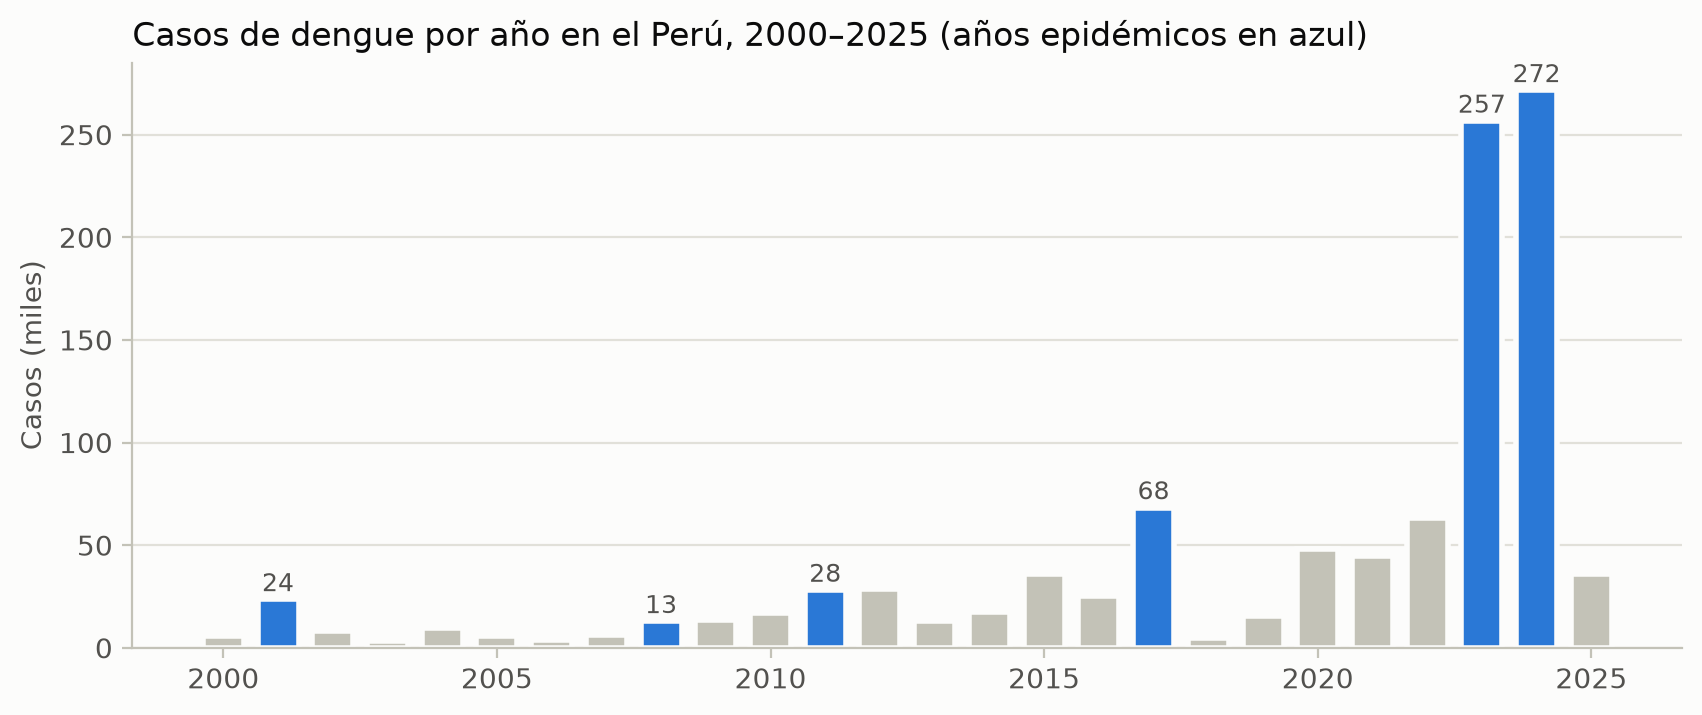
\includegraphics[width=0.72\textwidth]{q1_cases_per_year}
\caption{Casos de dengue por año, 2000–2025. En azul, los años epidémicos.}
\label{fig:q1}
\end{figure}

\paragraph{Q2 · Mayor incidencia.} El distrito con mayor incidencia fue La Huaca (Paita, Piura): 4,228 casos por
100,000 habitantes al año, unas 4 de cada 100 personas (Figura~\ref{fig:q2}). Se excluyeron los distritos con
menos de 10,000 habitantes, donde pocos casos producen tasas extremas. 10 de los 15 distritos con más incidencia
están en la costa, sobre todo en Piura y Áncash.

\begin{figure}[!htbp]
\centering
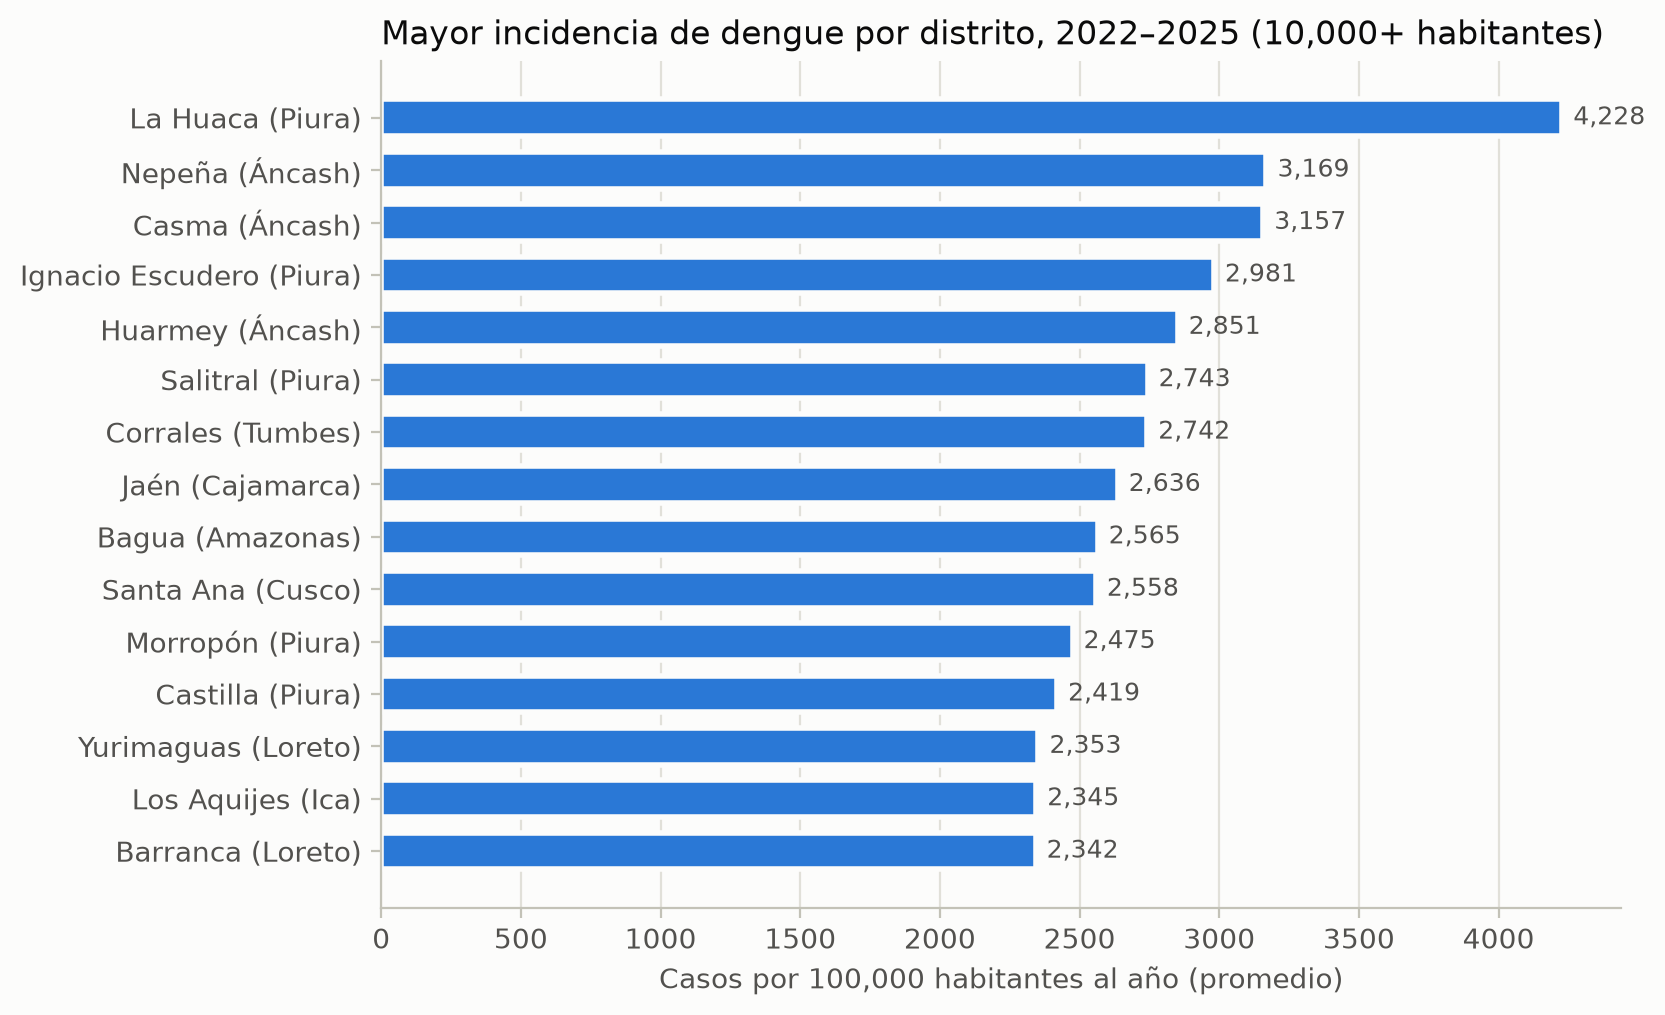
\includegraphics[width=0.5\textwidth]{q2_top_districts}
\caption{Los 15 distritos con mayor incidencia promedio, 2022–2025 (10,000 habitantes o más).}
\label{fig:q2}
\end{figure}

\paragraph{Q3 · Edad y sexo.} La incidencia más alta está en los adolescentes de 12 a 17 años, y las mujeres
superan a los hombres (479 frente a 405 casos por 100,000 al año) por las mujeres adultas
(Figura~\ref{fig:q3}). Los adultos de 30 a 59 años tienen más casos que cualquier otro grupo, pero solo porque es
el grupo con más población: por persona, su riesgo es igual al promedio nacional.

\paragraph{Q4 · Gravedad y establecimientos.} No hay relación. Los distritos con al menos 30 casos se dividieron
en cuatro grupos iguales según sus establecimientos activos por 10,000 habitantes (\code{ntile(4)}). La
proporción de casos con signos de alarma o graves es casi la misma en todos, entre 10\% y 13\%
(Figura~\ref{fig:q4}), y la correlación entre distritos es prácticamente nula ($r = 0.07$). La pequeña diferencia
va al revés de lo esperado: es algo mayor donde hay más establecimientos, probablemente porque ahí se detectan
mejor los signos de alarma.

\begin{figure}[!htbp]
\centering
\begin{subfigure}[b]{0.52\textwidth}
  \centering
  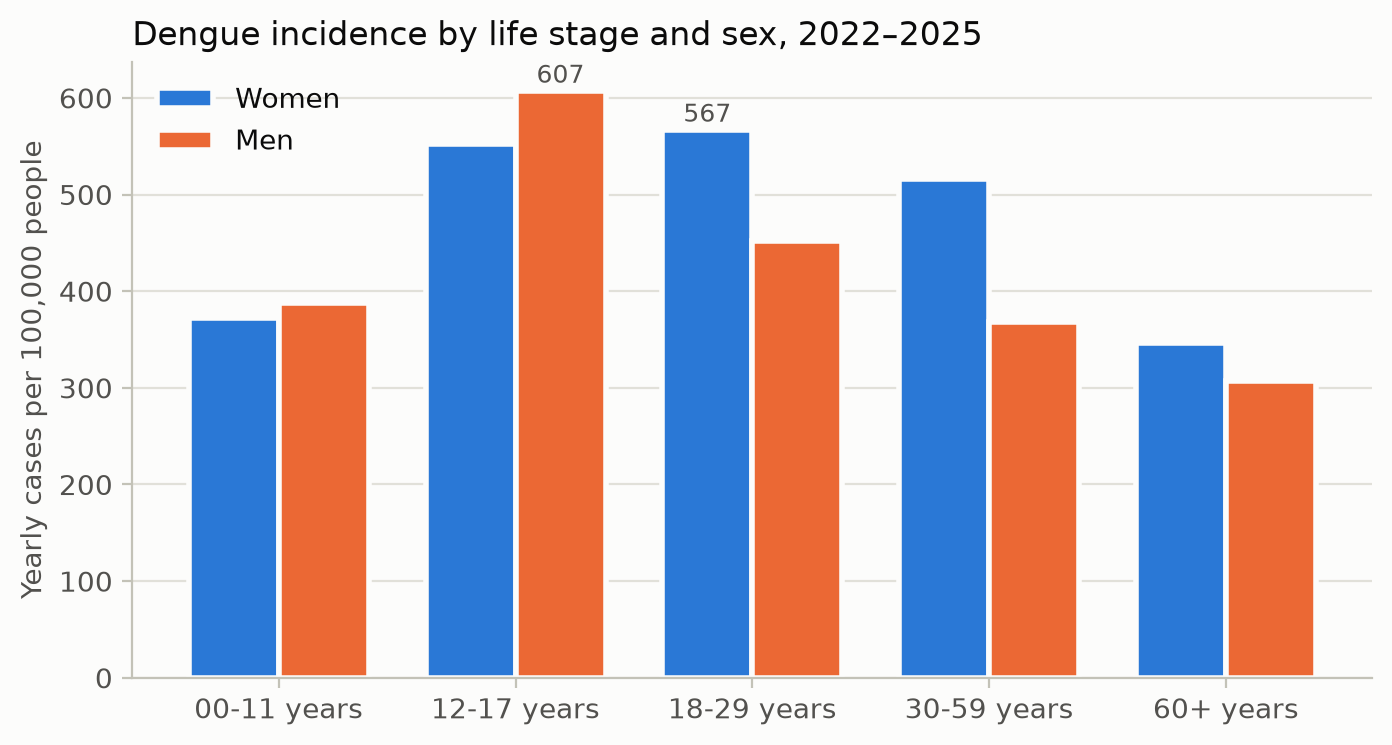
\includegraphics[width=\textwidth]{q3_age_sex}
  \caption{Q3: incidencia por etapa de vida y sexo.}
  \label{fig:q3}
\end{subfigure}\hfill
\begin{subfigure}[b]{0.46\textwidth}
  \centering
  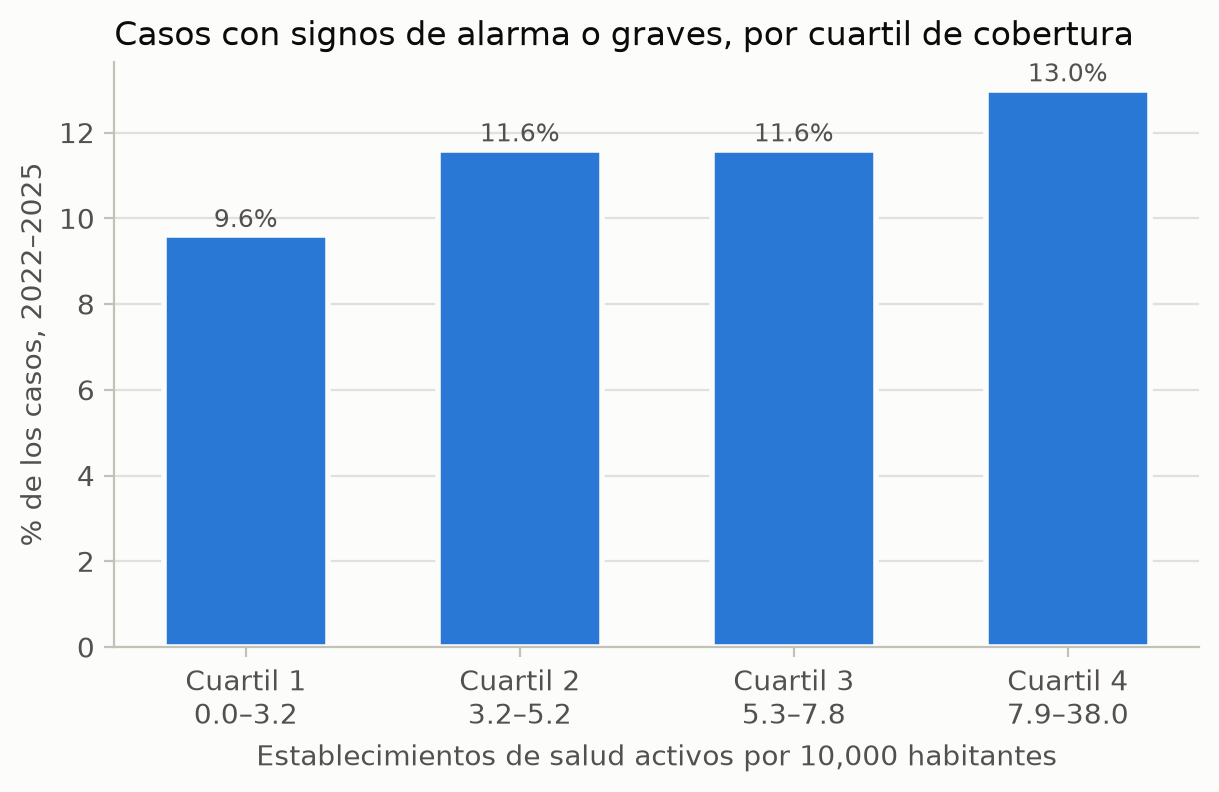
\includegraphics[width=\textwidth]{q4_severity_coverage}
  \caption{Q4: casos con signos de alarma o graves.}
  \label{fig:q4}
\end{subfigure}
\caption{Incidencia por grupo de población (Q3) y gravedad según la cobertura de establecimientos (Q4).}
\end{figure}

\paragraph{Q5 · Emergencias hídricas.} Sí, en las emergencias por lluvias. En los departamentos con al menos
1,000 casos en el año, los distritos en emergencia por lluvias tuvieron 2.3 veces más incidencia que los
distritos sin decreto en 2023, y 1.4 veces más en 2024 (Figura~\ref{fig:q5}). Las emergencias por déficit hídrico
no muestran ese aumento: se declararon sobre todo en departamentos andinos, donde casi no hay dengue. Entre los
distritos con decreto, los que tienen menos de 12 horas de agua al día tuvieron 3 veces más incidencia que los que
tienen entre 12 y 23 horas.

\begin{figure}[!htbp]
\centering
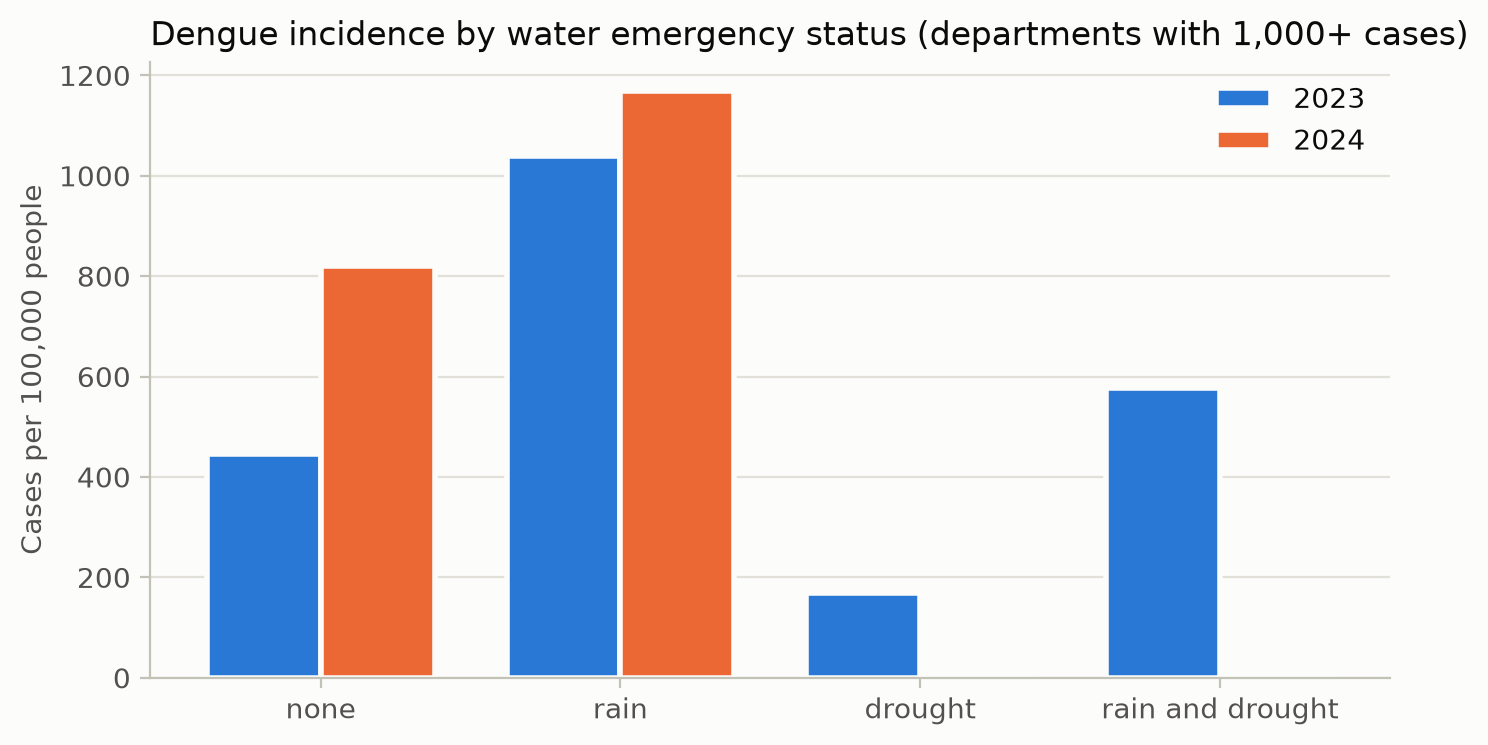
\includegraphics[width=0.5\textwidth]{q5_water_emergencies}
\caption{Incidencia según el tipo de emergencia hídrica del distrito, 2023 y 2024.}
\label{fig:q5}
\end{figure}

\paragraph{Q6 · Lluvia y casos.} Para cada estación se calculó la correlación entre la lluvia de la semana $t$ y
$\log(1 + \text{casos})$ de su provincia en la semana $t + k$, con $k$ de 0 a 12 semanas. El logaritmo evita que
las pocas semanas de pico, con miles de casos, decidan toda la correlación. En la costa, los casos aumentan entre
7 y 10 semanas después de la lluvia, con una relación moderada ($r$ de 0.26 a 0.44; Figura~\ref{fig:q6}): en
Piura, tras las lluvias de febrero a abril de 2023, los casos llegaron a su pico en mayo. En la selva no hay un
desfase claro ($r \le 0.26$): allí llueve todo el año, así que la lluvia no marca cuándo empieza un brote.

\begin{figure}[!htbp]
\centering
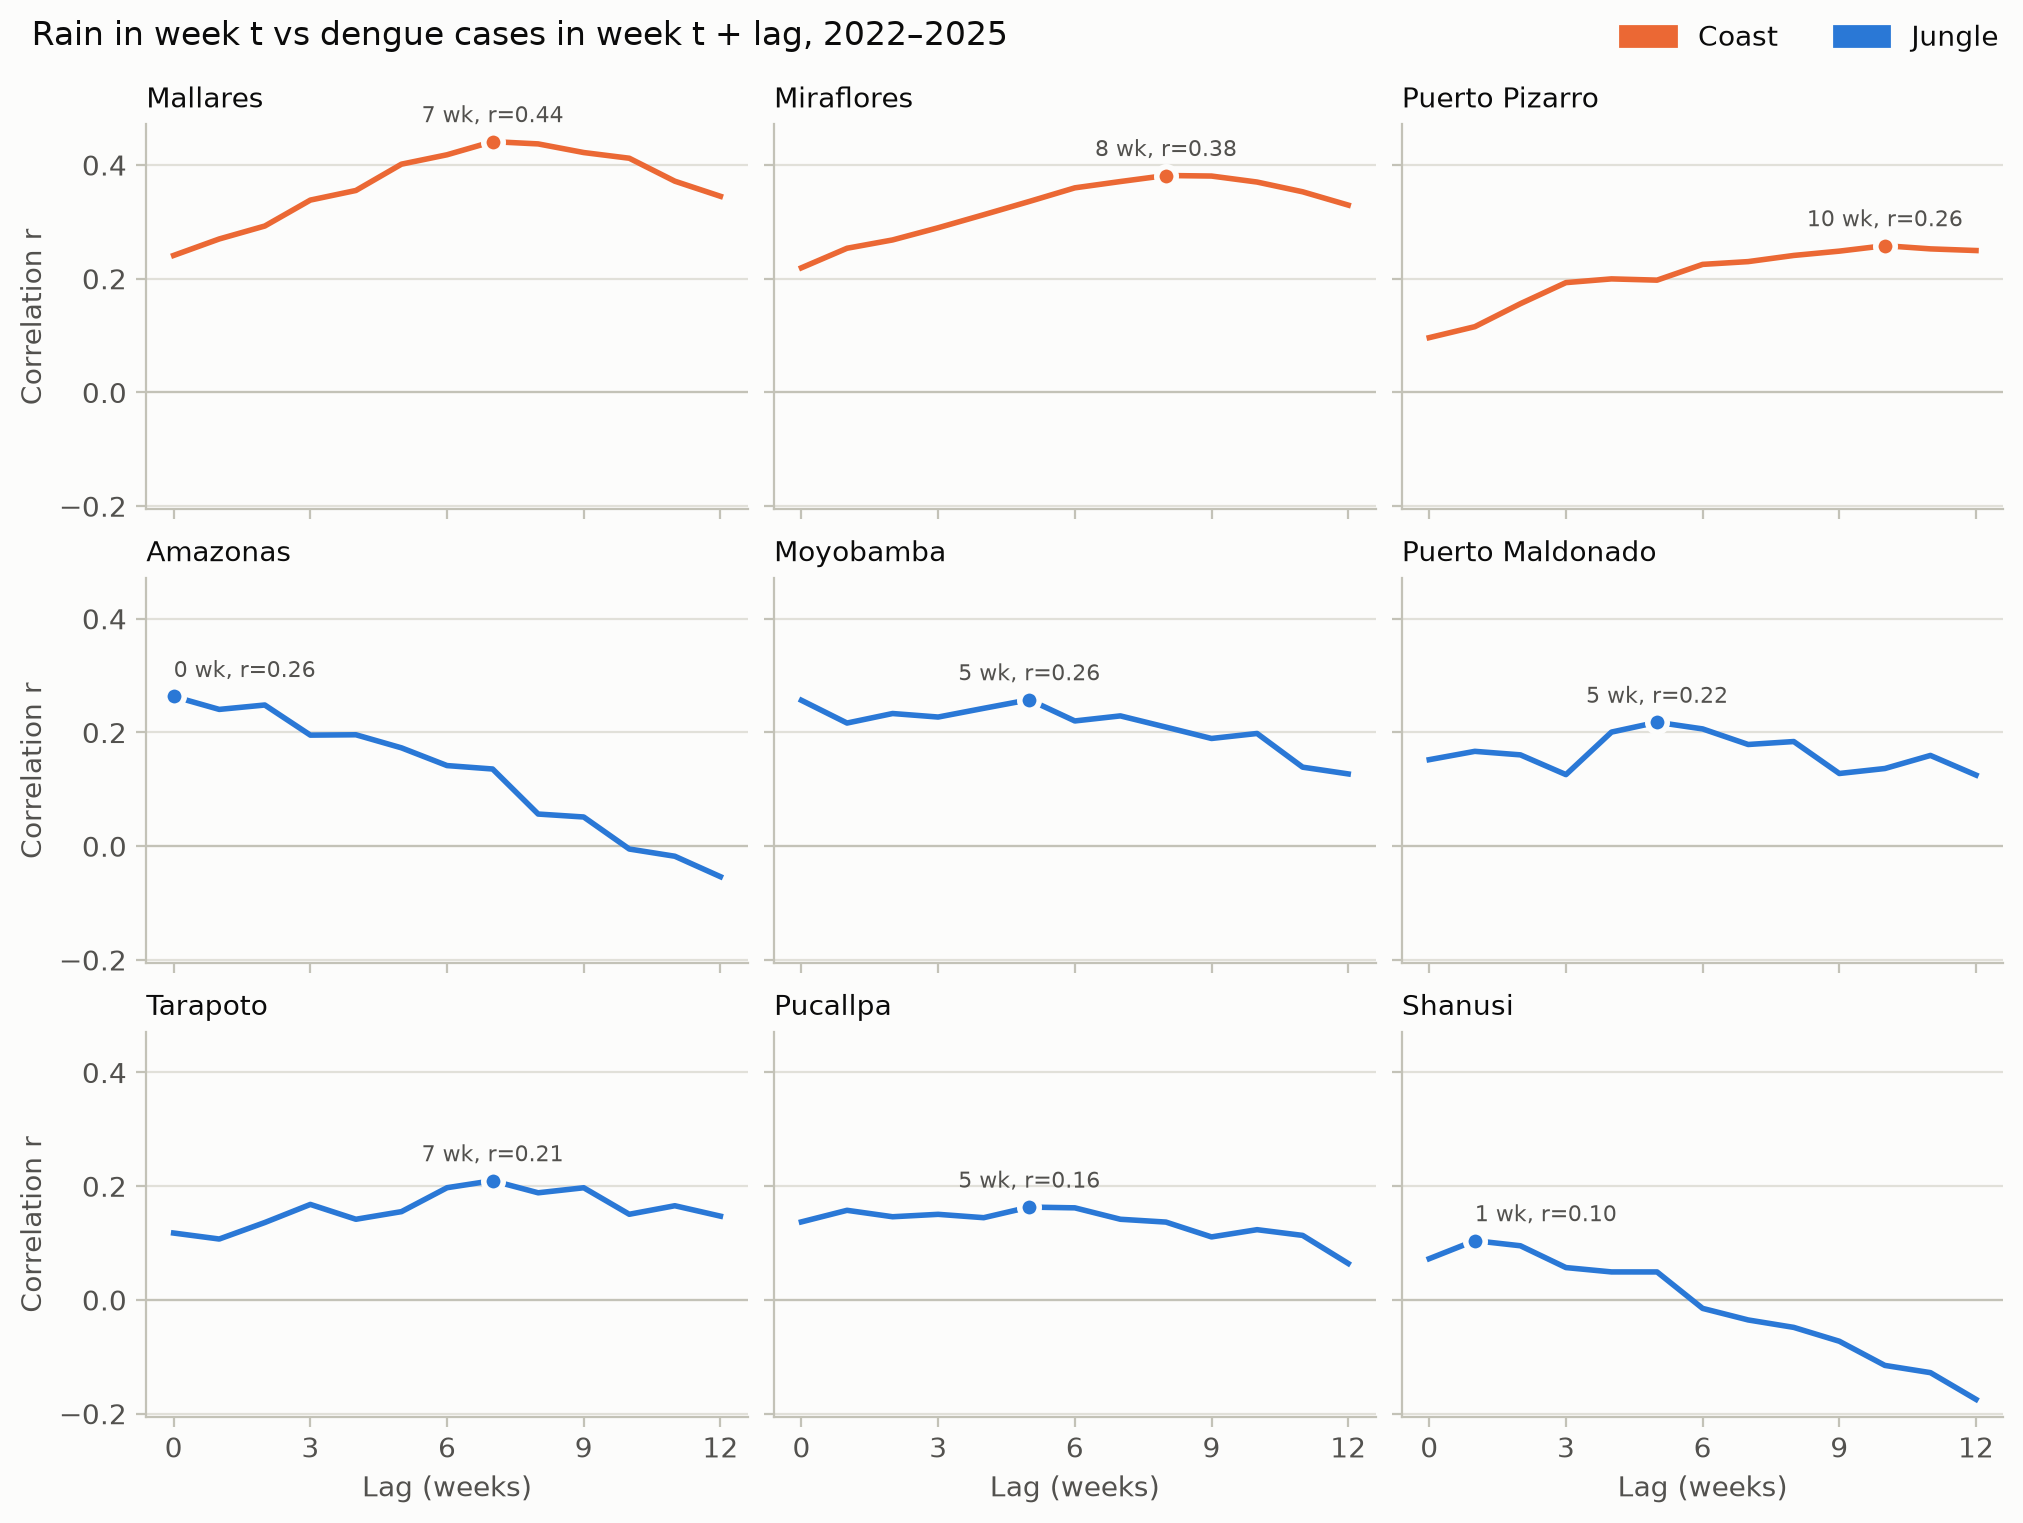
\includegraphics[width=0.56\textwidth]{q6_rain_lag_by_station}
\caption{Correlación entre la lluvia de la semana $t$ y los casos de la semana $t$ + desfase, por estación.}
\label{fig:q6}
\end{figure}

\paragraph{Limitaciones.} Los resultados son asociaciones, no relaciones causales. La población es la registrada
con DNI y no la censal; los establecimientos son un corte de 2026 frente a casos de 2022–2025; y las estaciones
tienen semanas sin datos, por lo que solo se usan las semanas con al menos 5 días medidos.
